\section{Ukázky detekce chodců}
\subsection*{Detekce ve videosekvenci s~konfigurací 15}
Testovací video je z~testovací sady \cite{testvideo}.
\begin{figure}[H]
\centering
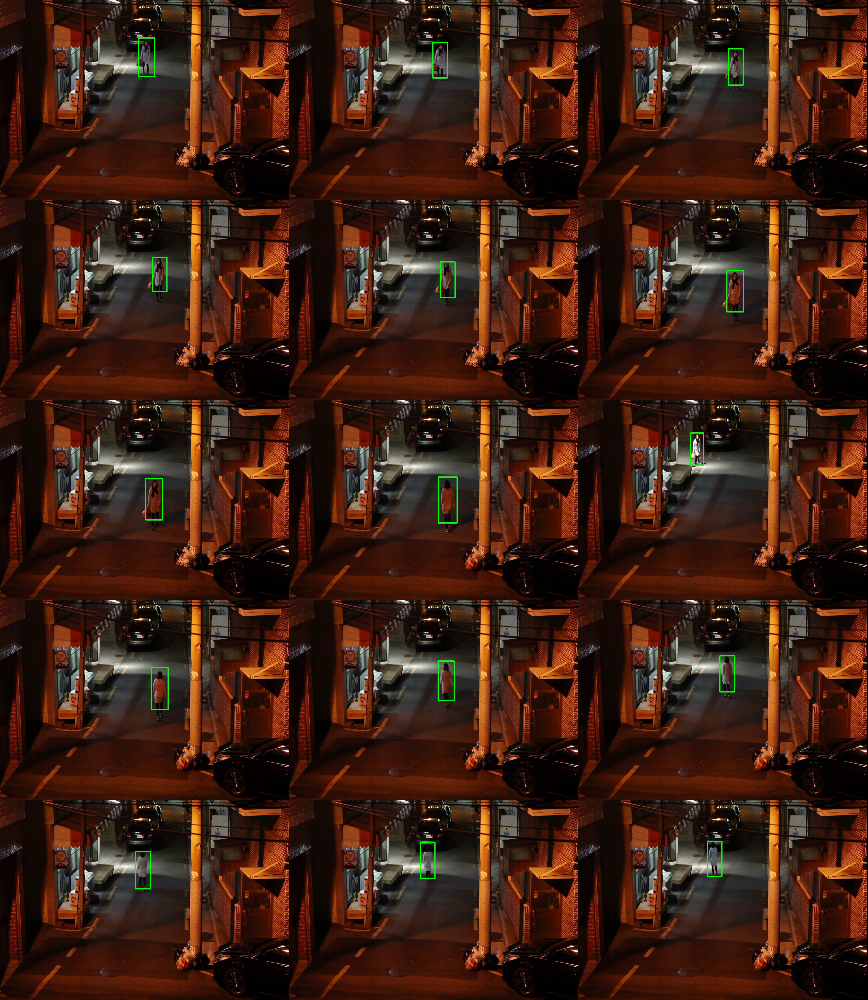
\includegraphics[keepaspectratio,width=16.5cm]{figures/videoMosaic}
\label{appVideo}
\end{figure}
\newpage
\subsection*{Detekce na obrázcích s~konfigurací 15}
Obrázky jsou z~testovací sady \cite{testimg}.
\label{appFigure}
\begin{figure}[H]
\centering
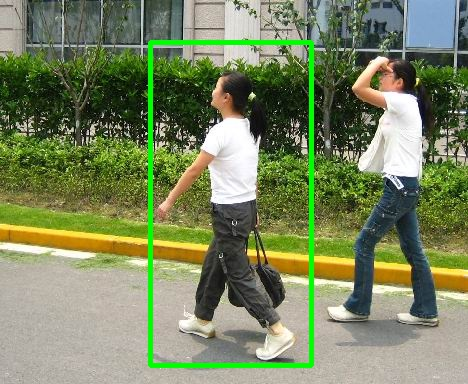
\includegraphics[keepaspectratio, max height=4.5cm,]{figures/ped/d/1}%
\hfill % <-- Seperation
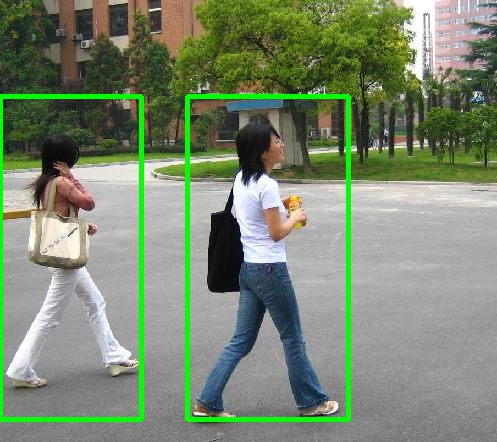
\includegraphics[keepaspectratio, max height=4.5cm,]{figures/ped/d/2}%
\hfill % <-- Seperation
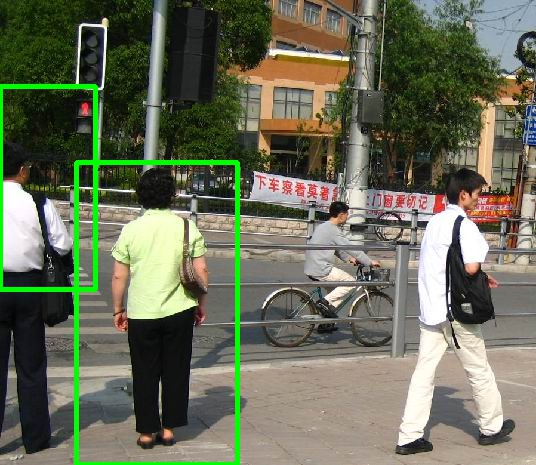
\includegraphics[keepaspectratio, max height=4.5cm,]{figures/ped/d/3}%
\end{figure}

\begin{figure}[H]
\centering
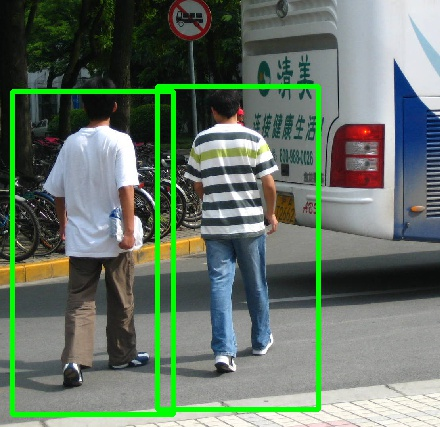
\includegraphics[keepaspectratio, max height=4.5cm,]{figures/ped/d/4}%
\hfill % <-- Seperation
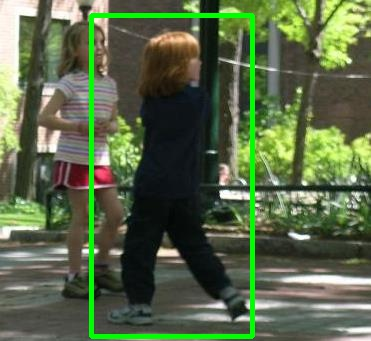
\includegraphics[keepaspectratio, max height=4.5cm,]{figures/ped/d/5}%
\hfill % <-- Seperation
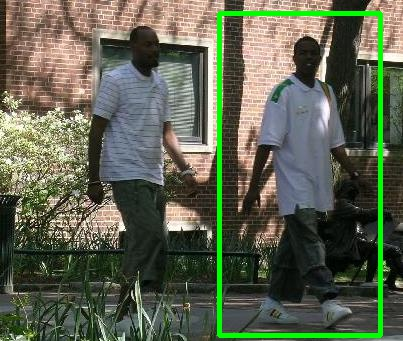
\includegraphics[keepaspectratio, max height=4.5cm,]{figures/ped/d/6}%
\end{figure}

\begin{figure}[H]
\centering
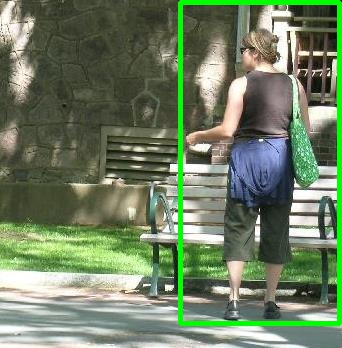
\includegraphics[keepaspectratio, max height=4.5cm,]{figures/ped/d/7}%
\hfill % <-- Seperation
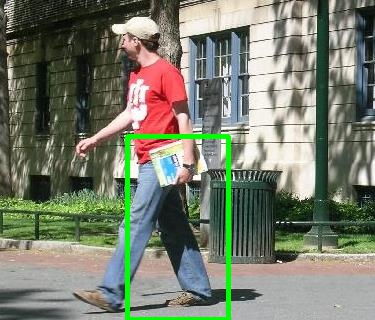
\includegraphics[keepaspectratio, max height=4.5cm,]{figures/ped/d/8}%
\hfill % <-- Seperation
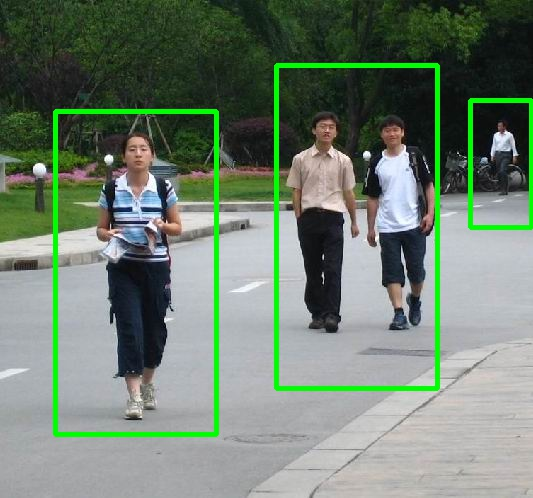
\includegraphics[keepaspectratio, max height=4.5cm,]{figures/ped/d/9}%
\end{figure}

\begin{figure}[H]
\centering
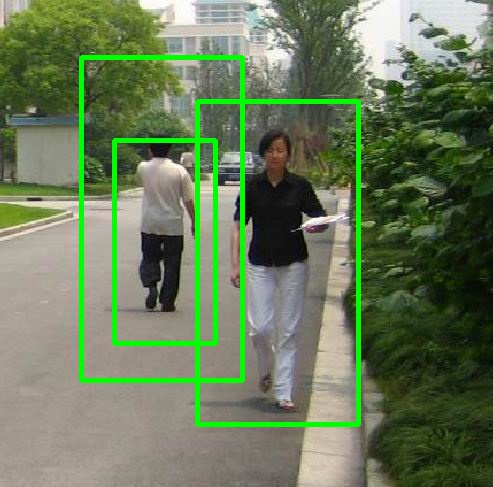
\includegraphics[keepaspectratio, max height=4.5cm,]{figures/ped/d/10}%
\hfill % <-- Seperation
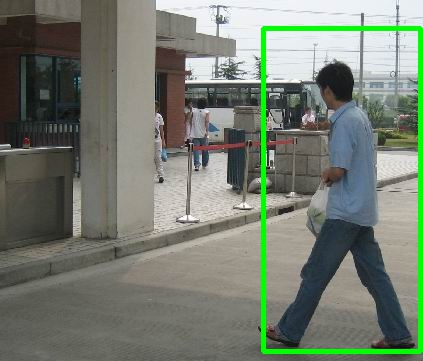
\includegraphics[keepaspectratio, max height=4.5cm,]{figures/ped/d/11}%
\hfill % <-- Seperation
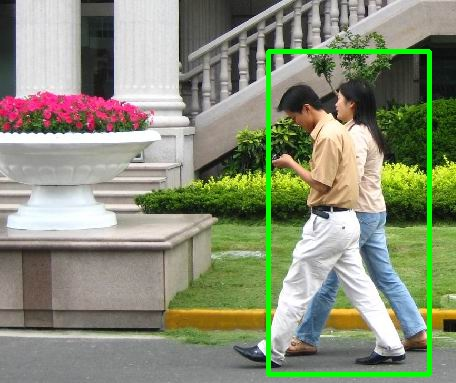
\includegraphics[keepaspectratio, max height=4.5cm,]{figures/ped/d/12}%
\end{figure}

\newpage
\section{Obsah přiloženého CD}
\subsubsection*{Struktura adresáře}
\dirtree{%
.0 project.
.1 apps.
.1 data.
.2 settings.
.2 tested.
.2 trained.
.1 docs.
.1 exDataset.
.1 samples.
.2 negative.
.2 positive.
.1 source.
.1 video.
}
\hfill \break
Součastí jsou i vytrénované klasifikátory z knihovny OpenCV (KONF\_15.yml) a Dlib (pedDet.svm).
\paragraph*{Apps}
Ve složce apps jsou umístěné skripty pro generování ROC křivek, textové soubory s~pravděpodobnostním zařazením a~výsledky křížové validace, resp. testování klasifikátoru. 
\paragraph*{Data}
Zde se nacházejí soubory s~nastavením, anotační soubory videí a~obrázků a~složku tested, kde se ukládá výstup detektoru.
\paragraph*{Docs}
Zde je umístěna programátorská dokumentace. Spouštění se provádí skrze soubor s~názvem index.html.
\paragraph*{ExDataset}
Zde jsou ukázky použitých datasetů.
\paragraph*{Samples}
Zde jsou soubory s~cestami k~negativním a~pozitivním vzorkům.
\paragraph*{Source}
Zde se nachází zdrojový kód implementované aplikace.
\paragraph*{Video}
Zde jsou umístěné videosekvence určené k~testování.

\subsection*{Uživatelská příručka}
\label{manual}
Stručnou nápovědu k~této aplikaci také získáme spuštěním s~argumentem \textbf{-h} nebo \textbf{-help}.
\subsubsection*{Spuštění detekce}
Aplikace dokáže detekovat ze tří druhů zdrojů, z~videa, obrázků a~webové kamery. Detekce ve videosekvenci se spustí argumentem \textbf{-v=<cesta-k-souboru>}, detekce z~webové kamery \textbf{-c=<číslo-zařízení>} a~z~obrázků \textbf{-i=<cesta-k-souboru-s-obrázky>}. Spuštění detekce s~vlastním detektorem vyžaduje další argumenty a~to \textbf{-class=<cesta-ke-klasifikátoru>} a~pro soubor s~jeho nastavením \textbf{-st=<cesta-k-souboru>}. Argumentem \textbf{-viz=1} povolíme náhled detekce.  Například spuštění detekce může vypadat takto: 
\begin{center}
\verb|./Pedestrian -v=video/cctv4_640.mp4 -class=KONF_15.yml| 
\verb|-settings=data/settings/settings_640.txt -viz=1|
\end{center}
\subsubsection*{Trénování klasifikátoru}
Trénování spustíme argumentem \textbf{-type=train}. Po spuštění aplikace s~tímto argumentem bude uživatel vyzván, aby vybral typ trénování. Nastavení pro trénování se nachází externě mimo program v~souboru. Pokud aplikaci nespustíme s~argumentem \textbf{-st=<cesta-k-souboru>}, načte se nastavení z~výchozího souboru \textit{settings.txt}. Argumentem \textbf{-verbose=1} vytiskneme aktuální nastavení trénovacích parametrů před trénovacím procesem.
\subsubsection*{Testování, křížová validace klasifikátoru}
Aplikace také disponuje testováním a~křížovou validací klasifikátoru, tu spustíme argumentem \textbf{-type=test}. Uživatel následně je vyzván k~výberu testování. Aplikace zvládá křížovou validaci klasifikátorů z~knihovny OpenCV i~z~knihovny Dlib. Pro testování nabídne pouze klasikátor z~knihovny OpenCV. 
\subsubsection*{}
\subsubsection*{Tvorba negativních vzorků}
Nástroj se spouští argumentem \textbf{-cs=<cesta-k-souboru-se-snímky>}. Po spuštění začne okamžitě pracovat. Snímky ukládá do složky \uv{makedSamples} a~po dokončení vypíše do konzole dobu trvání procesu. Velikost okna se definuje v~externím souboru nastavení, pokud chceme definovat velikost řezu, musíme nástroj spustis společně s~\textbf{-st=<cesta-k-souboru>}.
\subsubsection*{Anotační nástoj}
Nástroj se spouští argumentem \textbf{-e=<název-videa>}, po spuštění je uživatel dotázán, kolik osob bude anotovat (nanejvýš lze až 5 osob).
Klávesami `0' až `4' se přepíná mezi anotacemi, přičemž se tato selekce vypíše pro kontrolu do konzole. Klávesa `r' slouží pro vynulování vybrané anotace. Klávesou `n' přeskočíme aktuální snímek bez uložení anotovaných pozic. Klávesa `s' uloží aktuální anotované pozice do paměti a~přepne se na další snímek, přičemž pozice první anotace zůstane nezměněná, to umožňuje jednodušší práci, pokud se v~obraze nachází pouze jeden chodec. Klávesy `i', `j', `k' a~`l' umožňuje pohyb v~obraze, pro přesnější umístění anotované části. Pokud tyto klávesy stiskneme společně s~klávesou `shift', umožní nám to měnit velikost aktuálně vybrané anotace. Klávesa `x' uloží aktuální pozice anotací v~paměti do souboru. Tato funkcionalita umožňuje přerušovanou práci na anotacích videosekvence, ale vyžaduje manuální úpravu souboru uživatelem. Po posledním snímku z~videa se nástroj ukončí a~soubor s~anotacemi se uloží na disk se stejným názvem jako bylo zpracovávané video. Soubor je kompatibilní s~jakýmkoliv textovým editorem.